
\documentclass[journal]{IEEEtran}
\usepackage{blindtext}
\usepackage{graphicx}

\ifCLASSINFOpdf
  % \usepackage[pdftex]{graphicx}
  % declare the path(s) where your graphic files are
  % \graphicspath{{../pdf/}{../jpeg/}}
  % and their extensions so you won't have to specify these with
  % every instance of \includegraphics
  % \DeclareGraphicsExtensions{.pdf,.jpeg,.png}
\else
  % or other class option (dvipsone, dvipdf, if not using dvips). graphicx
  % will default to the driver specified in the system graphics.cfg if no
  % driver is specified.
  % \usepackage[dvips]{graphicx}
  % declare the path(s) where your graphic files are
  % \graphicspath{{../eps/}}
  % and their extensions so you won't have to specify these with
  % every instance of \includegraphics
  % \DeclareGraphicsExtensions{.eps}
\fi


\usepackage{CJK}
\usepackage[utf8]{inputenc}
\parindent=19pt

\renewcommand\thesection{\arabic{section}}

\renewcommand\thesubsection{\thesection.\arabic{subsection}}

\begin{document}


\renewcommand\thesection{\arabic{section}}

\renewcommand\thesubsection{\thesection.\arabic{subsection}}
%
% paper title
% can use linebreaks \\ within to get better formatting as desired
\begin{CJK}{UTF8}{gbsn}

\title{\textbf{TEEN:一种提高效率的无线传感网路由协议}}
%
%
% author names and IEEE memberships
% note positions of commas and nonbreaking spaces ( ~ ) LaTeX will not break
% a structure at a ~ so this keeps an author's name from being broken across
% two lines.
% use \thanks{} to gain access to the first footnote area
% a separate \thanks must be used for each paragraph as LaTeX2e's \thanks
% was not built to handle multiple paragraphs
%

\author{Arati Manjeshwar and Dharma P. Agrawal
\\Center for Distributed and Mobile Computing, ECECS Department,
\\University of Cincinnati, Cincinnati, OH 45221-0030
\thanks{This work is supported by the Ohio Board of Regents’ Doctoral Enhancement
Funds}% <-this % stops a space
\thanks{}% <-this % stops 
\thanks{}}

% The paper headers
\markboth{Journal of \LaTeX\ Class Files,~Vol.~6, No.~1, January~2007}%
{Shell \MakeLowercase{\textit{et al.}}: Bare Demo of IEEEtran.cls for Journals}


% make the title area
\maketitle


\begin{abstract}
无线传感器网络,预计在不久的将来找到广泛的适用性和得到越来越多的部署。在本文中,我们提出了一个正式的分类的传感器网络,基于其运作模式,分为主动式网络与反应式网络。反应式网络,相对于被动收集数据的主动网络,可以对快速变化的相关参数进行响应。我们针对反应式网络引入了一个新的节能协议,TEEN(阈值敏感的高效无线传感网协议)。我们用一个简单的温度传感应用来评估我们协议的性能。在能源效率方面,我们已经观察到此协议优于现有的传统传感器网络协议。
\end{abstract}

\IEEEpeerreviewmaketitle



\section{\textbf{引言}}
在最近几年中,一些应用正在提倡使用有线传感器网络。一些例子包括在某种结构中,例如飞机的关键位置部署的许多有线传感器,这样的条件使得能够从其内部和外部不断地进行监测,并且当监测设备即将失效时,可以发出及时的警报。

传感器网络通常是无人维护的,并且要有具有一定的容错性,因此其维护的代价应该是最小化的。特别是在这些应用中,传感器被嵌入到某种结构中或者放置在某些无法获得服务的荒凉地带。技术的进步使得我们有可能拥有体积小,低功耗的配备可编程计算模块,多参数传感模块,无线通信能力的设备。此外,低成本的传感器使得有可能拥有一个包含数百或数千个传感器的传感器网络,从而提高数据的可靠性和准确性以及覆盖率。传感器必须要易于部署(即不需要任何的安装成本等)。这些网络协议的设计必须遵从这样一种方式,即使得传感器在有限的功率内被有效地使用。另外,这些节点的操作和响应环境随着快速变化的物理参数是非常动态的。以下是一些基于其应用程序可以动态变化的一些参数:

\begin{itemize}
  \item 电力供应
  \item 位置(如果传感器节点是可移动的)  
  \item 可达性
  \item 任务类型(例如:传感器节点需要操作的属性)

\end{itemize}

因此,在这样的动态环境中,路由协议应该是容错的。传统的无线自组网路由协议适用性并不是很好,由于以下原因:

\begin{enumerate}
 \setcounter{enumi}
 \item 传感器网络是"以数据为中心",不同于传统网络的数据是从一个特定的节点请求,请求数据基于一定的属性,例如这一区域温度 \textgreater\ 50°F。
 \item 网络的要求随着应用程序的变化而变化,它是应用程序特定的。例如,在某些应用中,传感器节点是固定而不是移动的,而另一些需要基于一个属性(即属性是固定在这个网络)的数据。
 \item 相邻节点可能有类似的数据。因此,不是将数据分别从每个节点发送到请求的节点,而是理想的汇总类似的数据并发送它。
 \item 在传统的有线和无线网络中,每个节点都有一个独特的标识,用于进行路由。而不能有效地使用传感器网络。这是因为这些网络以数据为中心,从特定节点路由是不需要的。此外,在网络中的大量节点意味着需要大量检测,这可能远远大于实际数据传输的数量。

\end{enumerate}

 因此传感器网络需要的协议,是特定于应用程序的,以数据为中心的,并且能够聚集数据和优化能源消耗。一个理想的传感器网络应具有以下附加功能:
 
 在传感器网络中通常采用基于属性的寻址。属性地址是由一系列对某些指定的物理参数进行检测的属性值组成。例如,一个属性的地址可能是(温度 \textgreater\ 100°F,位置 = ??)。因此,所有的节点感知温度大于100°F应该返回它们的位置。

位置感知是另一个重要问题。由于大多数数据收集是基于位置的,节点需要在需要时知道自己的位置。


\section{\textbf{相关工作}}


在这一节中,我们简要介绍一些相关的研究工作。

Intanagonwiwat等人,[7]引入了一种数据传播范式称为传感器网络定向扩散。它是一个以数据为中心的范例,在这项工作中应用程序查询的传播和处理已被证明。


Estrin等人,[3]使用分层聚类方法对局部行为的重点,所需要的非对称通信和传感器网络中的能量进行了讨论。

一种基于簇的路由协议(CBRP)已经由Jiang等人,在[8]的移动自组织网络中提出。它使用分布式的方式将网络节点分成若干个重叠的或不相交的双跳集群。然而,这个协议不适合这种能量受限的传感器网络中使用。

Heinzelman等人,[5]介绍了层次聚类算法的传感器网络,称为LEACH。我们在6.1节更详细地讨论这个问题。


\section{\textbf{写作动机\\ }}

在无线传感器网络领域的研究工作中,我们看到对于目标应用程序的临界时间并没有特别的关注。大多数当前的协议假定传感器网络周期性地从它的环境收集数据或响应一个特定的查询以获得数据。我们觉得有必要引入一种对传感数据属性改变立即响应的网络。我们还认为,传感器网络应该向最终用户提供对能源效率,精度和动态响应时间综合调控的功能。因此在我们的研究中,我们一直专注于开发一个可以满足这些要求的通信协议。


\section{\textbf{传感器网络分类}}

在这里,我们提出了一种简单的基于传感器运作模式和目标应用程序类型的传感器网络分类。


\subsection{\textbf{主动式网络}}

网络中的节点周期性地对传感器和传输器进行切换,分别对环境数采集和对数据的进行传输。因此,该方法会定时对相关参数设置一个监测。它们非常适合需要定期监测数据的应用程序。

\subsection{\textbf{反应式网络}}

在这个方案中,节点会对突然变化的一个感测的属性进行响应。因此,它们非常适合于对时间准确性要求较高的应用。

\section{\textbf{传感器网络模型}}

我们现在考虑一种适合这些传感器网络的模型。它是基于Heinzelman等人[5]开发的模型。它由一个基站(BS),和若干远离基站的传感器节点组成,终端用户可以通过这个传感器网络获得数据。网络中的所有节点分布都是均匀的,并且最初具有相同的初始能量。同时基站有一个固定的电源供应器,因此没有能量的限制。它可以通过高功率信号向所有节点通信。因此不需要从基站路由到任何特定节点。然而,这些节点由于自身功率的约束,不能总是立刻直接回复基站,导致出现非对称通信现象。

这种模型采用了分层聚类方案。考虑图1所示的部分网络结构。每个集群都有一个簇头,它收集来自其群集成员的数据,将其聚集并发送给基站或上层簇头。例如,节点1.1.1,1.1.2,1.1.3,1.1.4,1.1.5和1.1形成一个集群,其中节点1.1作为簇头。类似地还有其他的簇头,如1.2,1等。这些簇头反过来组成了一个以节点1为簇头集群。因此,节点1也是一个二级簇头。这种模式重复形成一个具有层次的集群且最上层的集群节点直接向基站通信。基站成为了这个层次的根,并且监督整个网络。这种结构的主要特点是:

\begin{itemize}
  \item 所有节点只需要直接发送数据到它们的簇头,从而节省能量。
  \item 只有簇头需要进行额外的数据的计算。所以能量得到保留。 
\end{itemize}
\noindent
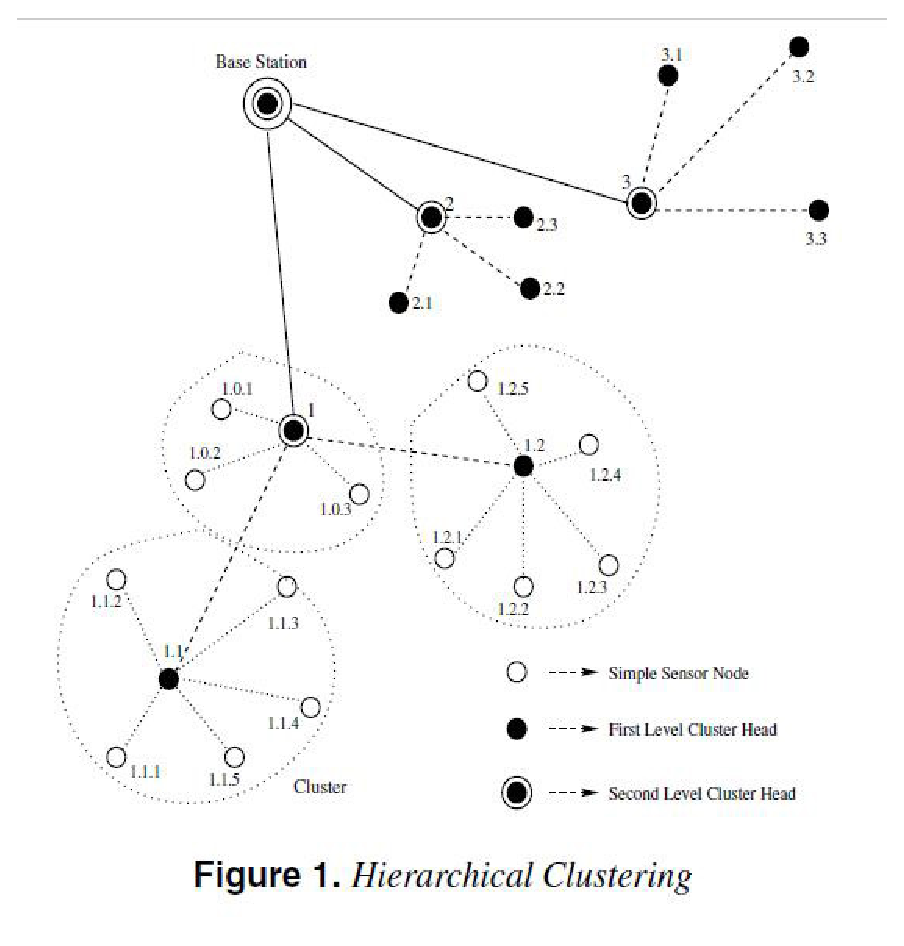
\includegraphics[height=250pt, width=250pt]{1.eps}

\begin{itemize}
  \item 在层次结构中的簇头需要在相对较大的距离上传输数据。结合它们执行额外的计算,最终消耗能源的速度比要其他节点更快。为了尽量将计算任务分散,所有的节点以一定的时间间隔,集群周期T轮流充当簇头。

\end{itemize}

\section{\textbf{传感器网络协议\\ \\ }}

在第5节中描述的传感器网络模型广泛使用了下面将要讨论的传感器网络协议。

\subsection{\textbf{主动式网络协议}}

在这一节中,我们讨论在主动网络协议中的功能和特性。
\\

\textbf{功能}

\

对于每个簇的变化时间,一旦簇头决定,簇头广播以下参数:

Report Time(TR):这是发送节点收到成功响应的时间间隔。

Attributes(A): 用户想要获取的数据的一组物理参数。

在每段响应时间内,群集成员监测属性中指定的参数并将数据发送到簇头。这种情况下簇头可能聚集这些数据,并将其发送到基站或更高级别的簇头。这确保用户拥有网络覆盖的整个区域的完整视图。 


\noindent
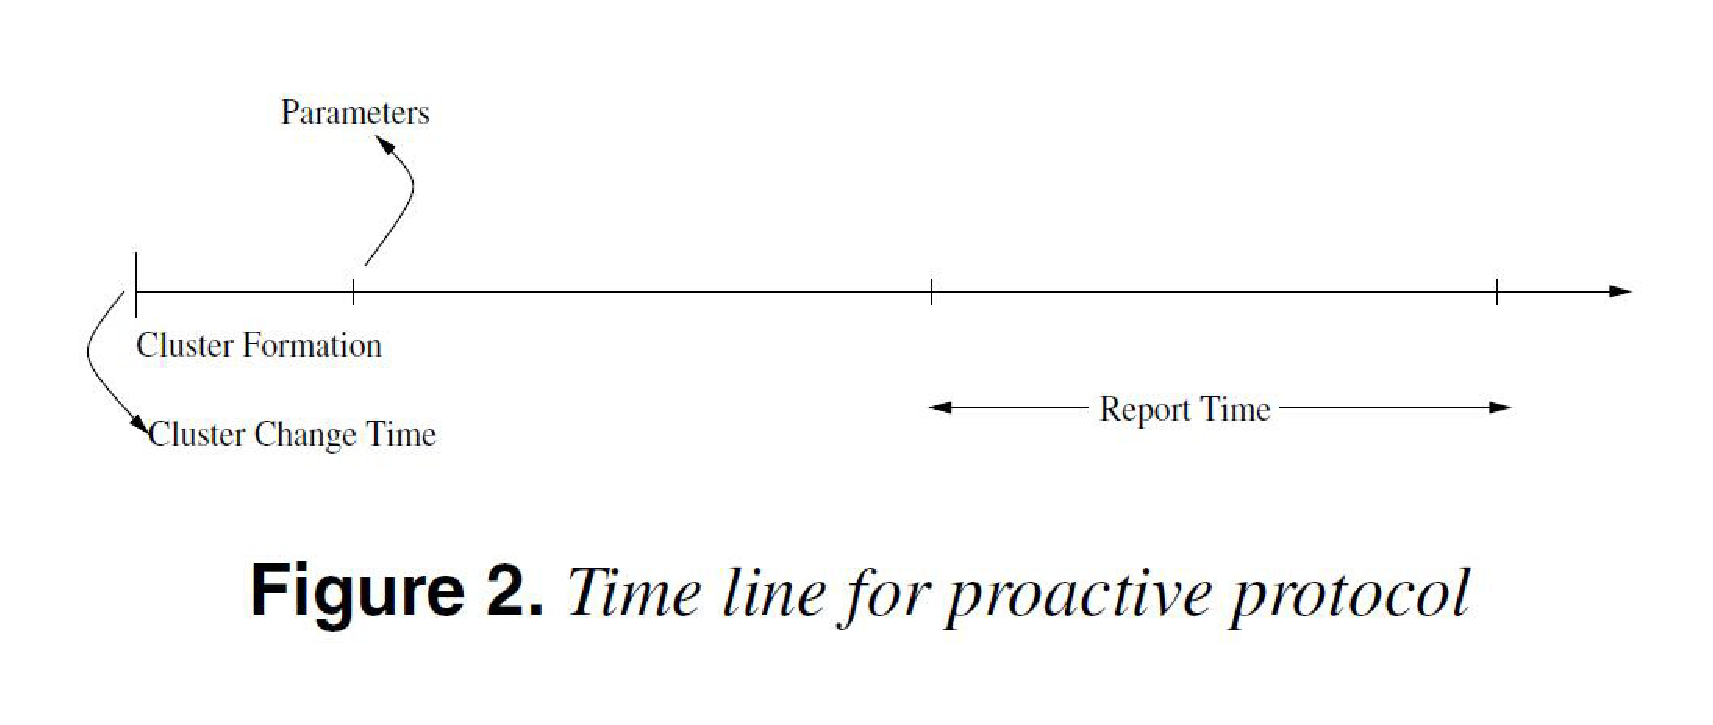
\includegraphics[height=100, width=250]{2.eps}

\textbf{重要特征}
\\*

这个方案的重要特点如下:
\\
\begin{enumerate}
 \setcounter{enumi}
 \item 由于节点在除了响应时间的其他所有时间内均关闭其传感器和数据传输器,所以其能量消耗很少。
 \item 在每一个集群改变时间内,TR和A通过重新传输进行刷新,因此它们是可以改变的。
 
\end{enumerate}

然而,这种方案有一个重要的缺点。由于数据被检测的周期性,可能时间同步数据在响应时间后到达用户端。因此,该方案可能不是非常适合于数据时间同步要求较高的传感器应用。

\

\textbf{LEACH}

\

LEACH (低能量自适应层次聚类) 是一种在[5]中提出的协议簇。LEACH是一个很好的类主动式网络协议,但是有一些小不同。

一旦簇形成,簇头广播TDMA调度命令使得群成员可以开始发送数据。完成这个调度所需的总时间称为帧时间TF。簇中的每个节点在发送数据到簇头的帧时间内都有其自己的时隙。当调度表中的最后一个节点已发送数据后,该调度表将刷新重复进行。

先前讨论的响应时间相当于LEACH的帧时间。帧时间不是由簇头广播,而是来自TDMA时间调度表。然而,它并不由用户控制。此外,该属性是预先确定的,并没有在中间改变。

\

\textbf{应用实例}

\

这个网络可以用来检测机械故障和对其进行诊断。它也可以用来在一个特定的地区收集温度变化数据。

\subsection{\textbf{反应式网络协议:TEEN}}

在这一节中,我们提出了一个新的网络协议称为TEEN协议(阈值敏感的能量高效传感器网络协议)。据我们所知,它是第一个针对反应式网络开发的网络协议。

\

\textbf{功能}

\



在这个方案中,在每个簇的变化时间内,除了属性,簇头还会将以下内容广播到它的成员:

\

硬门限(HT):这是检测到属性数据的阈值。它是一个绝对的值,如果节点检测的数据值超过它,那么必须打开数据传输器,并向簇头节点发送数据。

\

软门限(ST):这是检测数据属性值的一种小的变化,会触发节点打开它的数据传输器并开始传输。

\

节点持续地检测所处环境的数据。属性集第一次检测到一个参数达到它的硬门限时,该节点打开它的数据传输器并发送的检测到的数据。检测到的值存储在节点的一个内部变量中,称为检测值(SV)。节点将在当前集群周期内发送数据,只有在以下条件均成立时:

\begin{enumerate}
 \setcounter{enumi}
 \item 检测到当前的属性值大于硬门限。
 \item 所检测的属性值与SV的值之差等于或大于软门限。
 
\end{enumerate}

\noindent
当一个节点发送数据,SV设定等于监测属性的当前值。

因此,硬门限试图通过让节点只能在其数据属性值在有效范围内时才能传输数据来减少网络内的通信压力。软门限进一步降低了传输的数量,通过消除所有的微小变化或没有变化的数据属性的传输。

\noindent
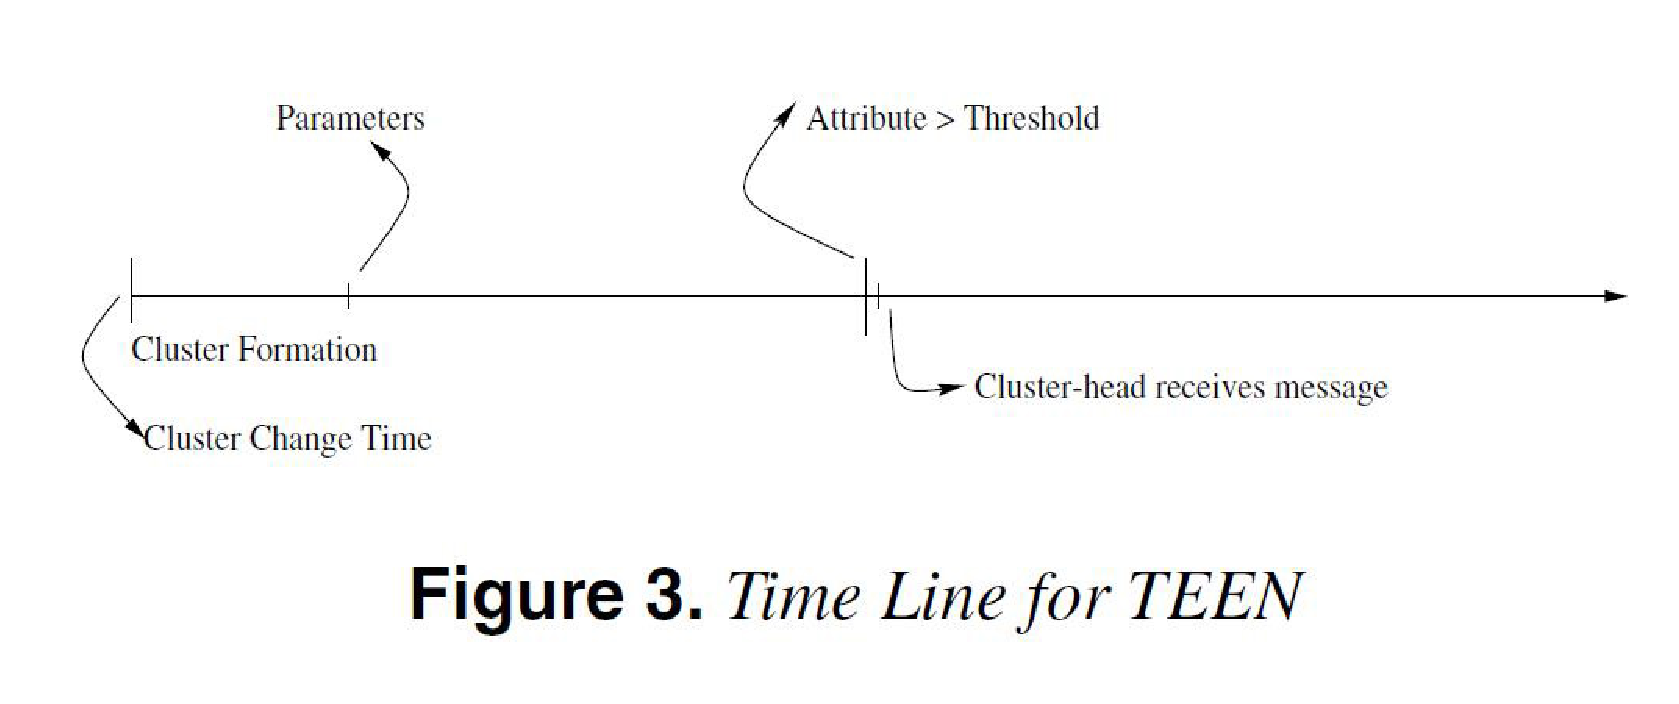
\includegraphics[height=100, width=250]{3.eps}

\textbf{重要特征}
\\*

这个方案的主要特点如下:
\\
\begin{enumerate}
 \setcounter{enumi}
 \item 时间关键的数据几乎瞬间到达用户端。
 \item 信息传输比数据监测消耗的能量要大得多。因此,尽管节点的不断地进行监测,在这个方案中的能量消耗可能会比主动式网络要小得多,因为数据传输并不经常进行。  \item 软门限可以是多样的,这取决于感测的属性和目标应用程序的主要关注点。
 \item 一个较小的软门限,在增加能量消耗的同时,给出了一个更准确的网络视图。因此,用户可以权衡控制能量效率和精度。
 \item 在每个簇的变化时间内,属性数据被会被重新广播,用户按照需求可以改变它们。
 \end{enumerate}

\

此方案的主要缺点是,如果没有达到阈值,节点间将永远不会进行通信,用户将不会得到任何来自网络的数据,即使所有节点失效,用户也根本不会知道。因此,该方案是不适合于用户需要在常规的基础上得到数据的应用程序。这个方案另一个可能的问题是,实际的实现时要确保在集群中没有碰撞。TDMA的节点调度可以避免这个问题。然而,这将引入一个延迟时间对于响应时间关键数据。CDMA是这个问题的另一种可能的解决方案。

\

\textbf{应用实例}

\

该协议是最适合于时间关键的应用,如入侵检测,爆炸检测等。

\section{\textbf{性能评估}}

\subsection{\textbf{模拟}}

为了对我们的协议的性能进行评估,我们已经在NS-2模拟器[10]上实现了LEACH[4]协议的扩展。我们进行模拟的目标如下:

\begin{itemize}
  \item 在能量消耗和网络寿命的基础上对TEEN和LEACH协议的性能进行比较。
  \item 研究软门限ST对TEEN协议的影响。  

\end{itemize}

模拟在一个拥有100个节点和一个固定的基站的网络上进行。节点随机放置在网络中。所有节点开始时拥有初始能量2J,集群以LEACH协议构造[5][6]。但是它们的无线传输模型被修改以包括空闲时间功耗(设置等于无线传输能量)和传感功耗(设置等于10\%的无线传输能量)。空闲时间的功耗在所有网络中被设置为相同的,其并不影响协议性能的比较。%的无线电电子能)。

\

\textbf{模拟环境}

\

在我们的实验中,我们模拟了不同地区的温度变化环境。传感器网络节点首先被随机放置在100x100单位的边界地区。网络覆盖的实际区域分为四个象限。每个象限之后在模拟的过程中每5秒被随机分配一个在0°F 到 200°F之间的的随机温度。我们观察到,大多数集群很好地分布到四个象限。

\

\textbf{实验}

\

我们使用两个指标来分析和比较协议的性能。它们为:

\

平均能耗:这个指标表示每个节点在网络中执行各种各样的功能时随时间平均消耗的能量,例如发送,接收,感知,和聚集数据等。

\

活跃节点的数量:这个指标表示网络的整体寿命。更重要的是,它给出了随着时间的推移网络的覆盖范围。

\

我们现在看看实现这些协议所使用的各种参数。协议的共同参数是被检测到的属性,温度。

对TEEN协议的性能进行了两种模式的研究,一种是只针对硬门限(硬模式),另一种是同时针对硬门限和软门限(软模式)。硬门限设定在最低和最高温度的平均值,100°F。软门限在我们的实验中设置为2°F。

\subsection{\textbf{结果}}

我们为每个协议和每个模式的TEEN协议运行了5个模拟器。从这5个试验读数,然后平均绘制。在任何特定的时间拥有一个较低的能耗度和更多的活跃节点,表示这是一个更有效的协议。

\noindent
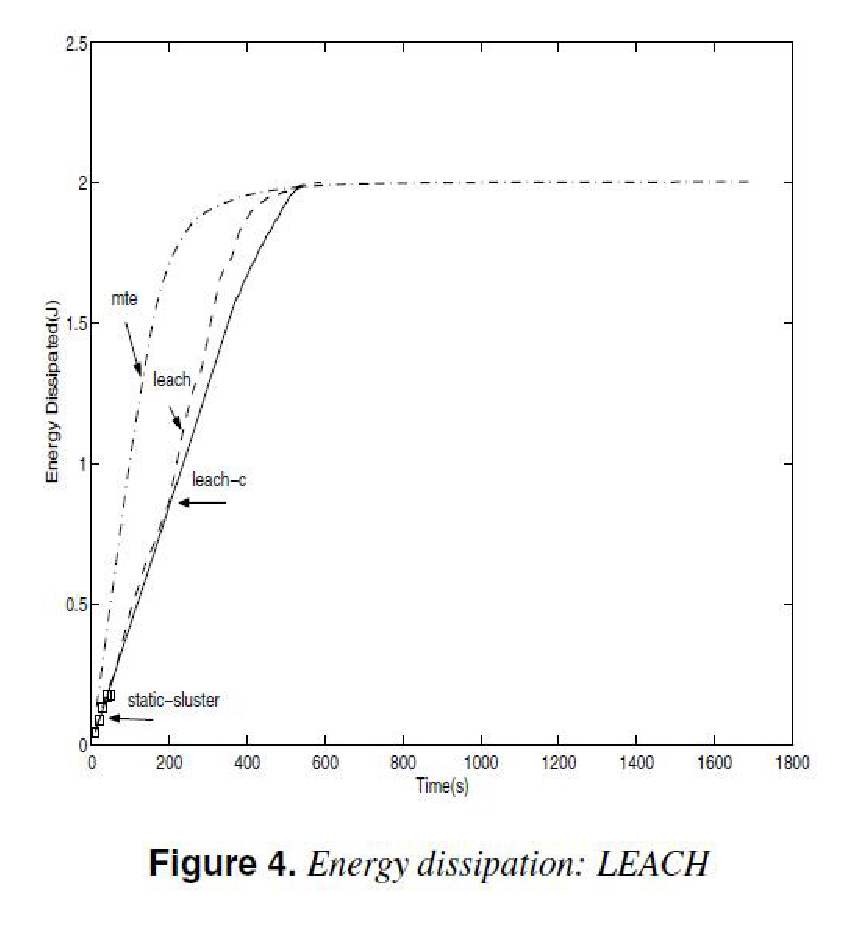
\includegraphics[height=260, width=250]{4.eps}

图4和图5显示了在主动模式下网络的行为。这种比较最初是在LEACH上实现[6]。考虑到修改后的无线传输能量模型在这里对其进行重复的说明。这四个协议[6]中,MTE(最小传输能量)的持续时间最长。然而,我们从图5中观察到只有1个或2个节点是真正处于活跃状态的。因此,LEACH和LEACH-C协议(LEACH协议的一个变种)在能量消耗和网络寿命方面可以被认为是最有效的协议。

在图6和图7中,我们比较了这两个协议。我们看到,这两种模式的TEEN协议的性能远优于LEACH协议。如果集群是基于LEACH-C协议组成的,TEEN协议的性能预计将表现的更好。

正如预期的那样,因为软门限的存在,软门限模式的TEEN协议性能远优于硬门限模式的TEEN协议。

\noindent
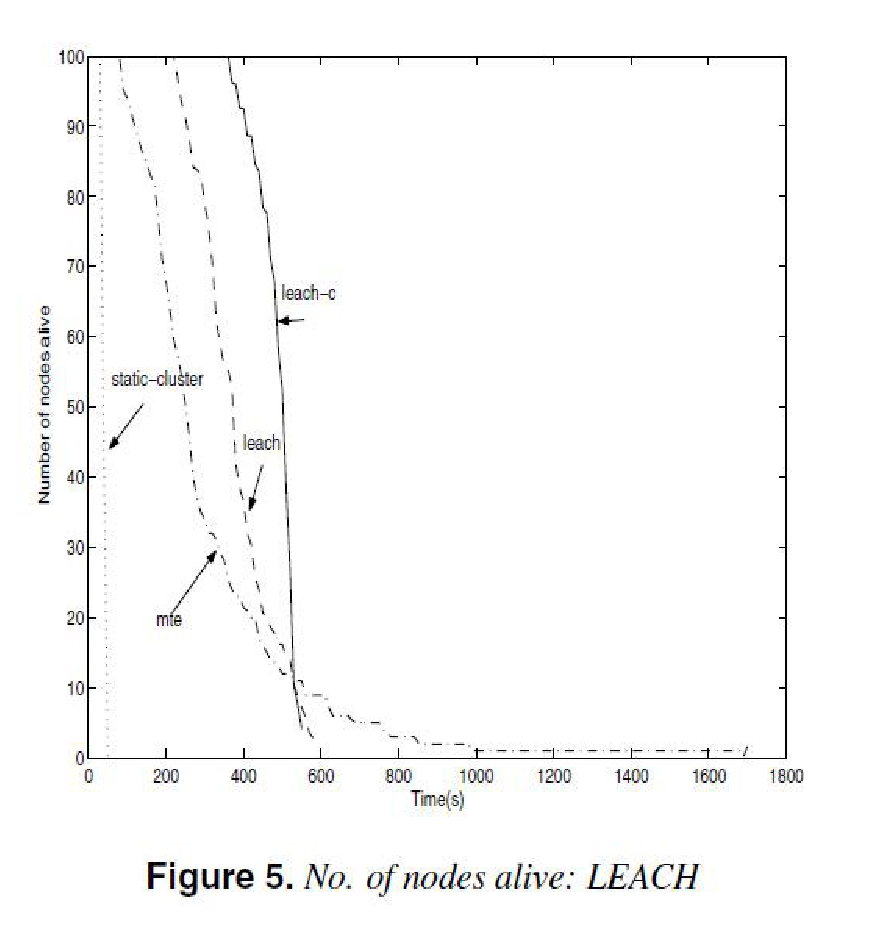
\includegraphics[height=260, width=250]{5.eps}

\noindent
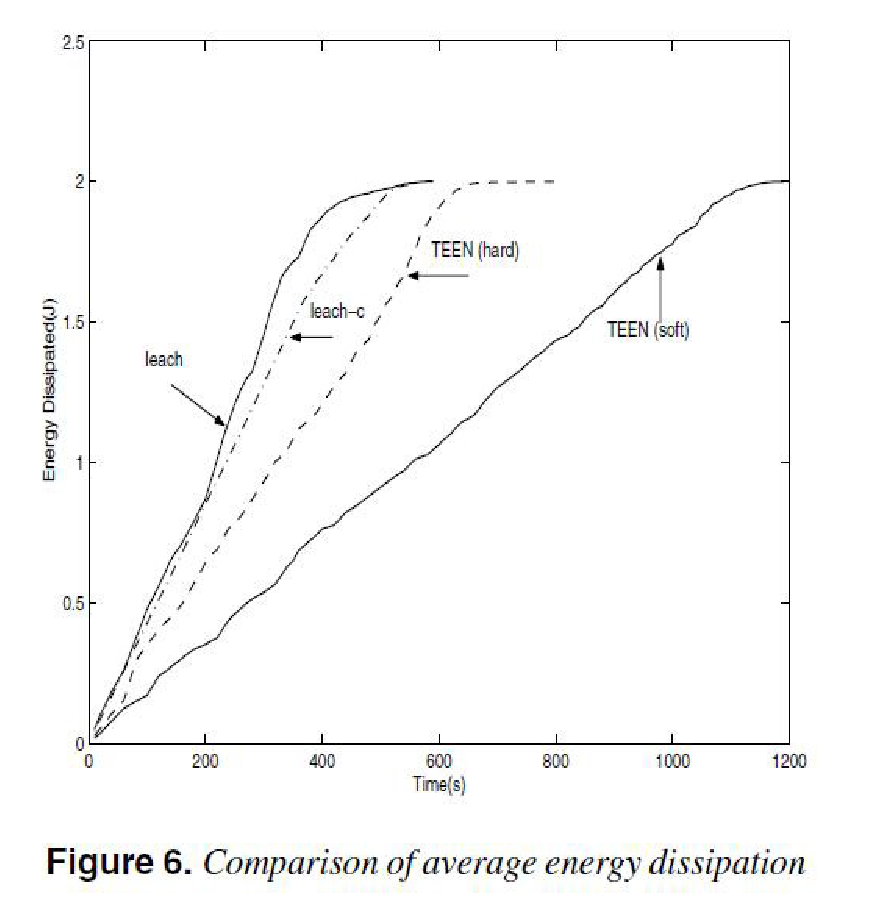
\includegraphics[height=260, width=250]{6.eps}

\noindent
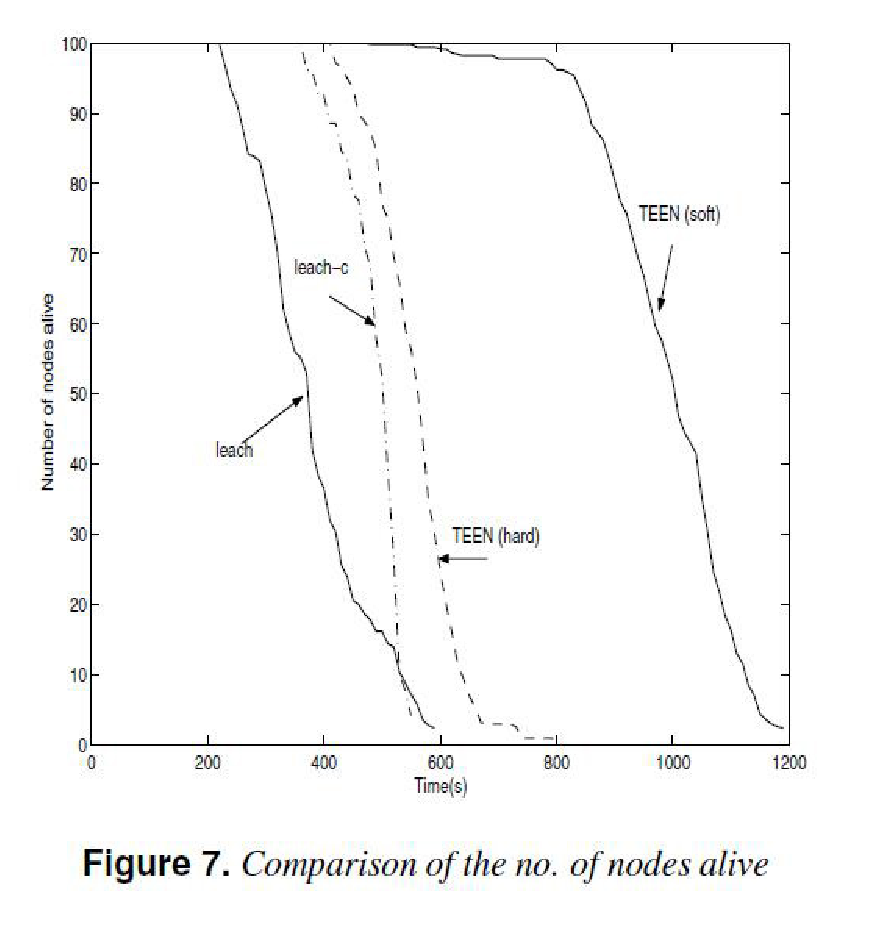
\includegraphics[height=260, width=250]{7.eps}

\section{\textbf{总结}}

在本文中,我们提出了一个正式的传感器网络分类。我们还引入了一个新的网络协议,反应式网络的TEEN协议。TEEN协议非常适合于时间关键的应用,在能量消耗和响应时间方面也非常高效。它还允许用户控制能耗和精度以适应具体的应用程序。

\section*{Acknowledgment}

我们要感谢Wendi Heinzelman的宝贵建议,以及允许我们使用她的LEACH延伸协议在NS上进行模拟实验。

% Can use something like this to put references on a page
% by themselves when using endfloat and the captionsoff option.
\ifCLASSOPTIONcaptionsoff
  \newpage
\fi



% trigger a \newpage just before the given reference
% number - used to balance the columns on the last page
% adjust value as needed - may need to be readjusted if
% the document is modified later
%\IEEEtriggeratref{8}
% The "triggered" command can be changed if desired:
%\IEEEtriggercmd{\enlargethispage{-5in}}

% references section

% can use a bibliography generated by BibTeX as a .bbl file
% BibTeX documentation can be easily obtained at:
% http://www.ctan.org/tex-archive/biblio/bibtex/contrib/doc/
% The IEEEtran BibTeX style support page is at:
% http://www.michaelshell.org/tex/ieeetran/bibtex/
%\bibliographystyle{IEEEtran}
% argument is your BibTeX string definitions and bibliography database(s)
%\bibliography{IEEEabrv,../bib/paper}
%
% <OR> manually copy in the resultant .bbl file
% set second argument of \begin to the number of references
% (used to reserve space for the reference number labels box)

\begin{thebibliography}{1}

\bibitem{IEEEhowto:kopka}
J. Broch, D. Maltz, D. Johnson, Y. Hu, and J. Jetcheva.
“A Performance Comparison of Multi-Hop Wireless Ad
Hoc Network Routing Protocols”. In Proceedings of the
Fourth Annual ACM/IEEE International Conference on Mobile
Computing and Networking(MOBICOM), ACM, October 1998.

\bibitem{IEEEhowto:kopka}
J. Elson and D. Estrin. “An Address-Free Architecture
for Dynamic Sensor Networks”. Technical Report 00-724,
Computer Science Department, USC, January 2000.

\bibitem{IEEEhowto:kopka}
D. Estrin, R. Govindan, J. Heidemann, and S. Kumar. “Next
Century Challenges: Scalable Coordination inWireless Networks”.
In Proceedings of the 5th Annual ACM/IEEE International
Conference on Mobile Computing and Networking(
MOBICOM), pages 263–270, 1999.

\bibitem{IEEEhowto:kopka}
W. Heinzelman, A. Chandrakasan, and H. Balakrishnan.
“uAMPS ns Code Extensions”. http://wwwmtl.mit.edu/research/icsystems/uamps/ leach.

\bibitem{IEEEhowto:kopka}
W. Heinzelman, A. Chandrakasan, and H. Balakrishnan. “Energy-Efficient Communication Protocols for Wireless
Microsensor Networks”. In Proceedings of Hawaiian International
Conference on Systems Science, January 2000.

\bibitem{IEEEhowto:kopka}
W. B. Heinzelman. “Application-Specific Protocol Architectures
for Wireless Networks”. PhD thesis, Massachusetts
Institute of Technology, June 2000.

\bibitem{IEEEhowto:kopka}
C. Intanagonwiwat, R. Govindan, and D. Estrin. “Directed
Diffusion: A Scalable and Robust Communication
Paradigm for Sensor Networks ”. In Proceedings of the
6th Annual ACM/IEEE International Conference on Mobile
Computing and Networking(MOBICOM), pages 56–67, August
2000.

\bibitem{IEEEhowto:kopka}
M. Jiang, J. Li, and Y. C. Tay. “Cluster Based Routing Protocol”.
Internet Draft, 1999.

\bibitem{IEEEhowto:kopka}
E. M. Royer and C.-K. Toh. “A Review of Current Routing
Protocols for Ad-Hoc Mobile Wireless Networks”. In
IEEE Personal Communications Magazine, pages 46–55,
April 1999.

\bibitem{IEEEhowto:kopka}
UCB/LBNL/VINT. “Network Simulator-ns”. http://wwwmash.
cs.berkeley.edu/ns.
\end{thebibliography}


\end{CJK}
% that's all folks
\end{document}

